\documentclass[]{elsarticle} %review=doublespace preprint=single 5p=2 column
%%% Begin My package additions %%%%%%%%%%%%%%%%%%%
\usepackage[hyphens]{url}
\usepackage{lineno} % add
\providecommand{\tightlist}{%
  \setlength{\itemsep}{0pt}\setlength{\parskip}{0pt}}

\bibliographystyle{elsarticle-harv}
\biboptions{sort&compress} % For natbib
\usepackage{graphicx}
\usepackage{booktabs} % book-quality tables
%% Redefines the elsarticle footer
%\makeatletter
%\def\ps@pprintTitle{%
% \let\@oddhead\@empty
% \let\@evenhead\@empty
% \def\@oddfoot{\it \hfill\today}%
% \let\@evenfoot\@oddfoot}
%\makeatother

% A modified page layout
\textwidth 6.75in
\oddsidemargin -0.15in
\evensidemargin -0.15in
\textheight 9in
\topmargin -0.5in
%%%%%%%%%%%%%%%% end my additions to header

\usepackage[T1]{fontenc}
\usepackage{lmodern}
\usepackage{amssymb,amsmath}
\usepackage{ifxetex,ifluatex}
\usepackage{fixltx2e} % provides \textsubscript
% use upquote if available, for straight quotes in verbatim environments
\IfFileExists{upquote.sty}{\usepackage{upquote}}{}
\ifnum 0\ifxetex 1\fi\ifluatex 1\fi=0 % if pdftex
  \usepackage[utf8]{inputenc}
\else % if luatex or xelatex
  \usepackage{fontspec}
  \ifxetex
    \usepackage{xltxtra,xunicode}
  \fi
  \defaultfontfeatures{Mapping=tex-text,Scale=MatchLowercase}
  \newcommand{\euro}{€}
\fi
% use microtype if available
\IfFileExists{microtype.sty}{\usepackage{microtype}}{}
\usepackage[margin=1in]{geometry}
\usepackage{graphicx}
% We will generate all images so they have a width \maxwidth. This means
% that they will get their normal width if they fit onto the page, but
% are scaled down if they would overflow the margins.
\makeatletter
\def\maxwidth{\ifdim\Gin@nat@width>\linewidth\linewidth
\else\Gin@nat@width\fi}
\makeatother
\let\Oldincludegraphics\includegraphics
\renewcommand{\includegraphics}[1]{\Oldincludegraphics[width=\maxwidth]{#1}}
\ifxetex
  \usepackage[setpagesize=false, % page size defined by xetex
              unicode=false, % unicode breaks when used with xetex
              xetex]{hyperref}
\else
  \usepackage[unicode=true]{hyperref}
\fi
\hypersetup{breaklinks=true,
            bookmarks=true,
            pdfauthor={},
            pdftitle={Short Paper},
            colorlinks=true,
            urlcolor=blue,
            linkcolor=magenta,
            pdfborder={0 0 0}}
\urlstyle{same}  % don't use monospace font for urls
\setlength{\parindent}{0pt}
\setlength{\parskip}{6pt plus 2pt minus 1pt}
\setlength{\emergencystretch}{3em}  % prevent overfull lines
\setcounter{secnumdepth}{0}
% Pandoc toggle for numbering sections (defaults to be off)
\setcounter{secnumdepth}{0}
% Pandoc header


\usepackage[nomarkers]{endfloat}

\begin{document}
\begin{frontmatter}

  \title{Short Paper}
    \author[Princeton University]{Galileu Kim}
   \ead{galileuk@princeton.edu} 
  
    
  \begin{abstract}
  This paper represents a first step in a larger research project on local
  state capacity and public goods delivery. It focuses on a particular
  dimension of state capacity, namely, its administrative capacity.
  Because of decentralization, municipal-level bureaucrats have increased
  in size and importance. However, this growing sector in the
  administrative structure of the developing countries across Latin
  America remains relatively unexplored. Building on a micro-level data
  set of municipal-level bureaucrats in Brazil from 1998 to 2015, the
  paper describes inter-municipal and inter-temporal variation in a key
  outcome of interest, the educational levels of bureaucrats in the
  executive branches of Brazilian municipalities. It then proposes an
  identification strategy for estimating the effect of partisanship on the
  staffing decisions made by mayors.
  \end{abstract}
  
 \end{frontmatter}

\subsection{Literature Review}\label{literature-review}

State capacity has been the subject of extensive research, especially in
the context of the developing world. Scholars have linked it to certain
outcomes such as economic development\footnote{Coatsworth 1998, Kurtz
  2013.} , the successful creation of a developmental state\footnote{Kohli
  2004.} and democratic stability.\footnote{O'Donnell 1993.} These
different works have converged in the importance of state capacity, but
in doing so have emphasized different dimensions of the
concept.\footnote{O'Donnell 1993.}

Some scholars analyzed the extractive capacity of the state: whether it
is able to exact financial contributions from its citizens.\footnote{Vom
  Haum and Soifer 2008, pp.~220.} Others have focused on administrative
capacity, analyzing the role of bureaucratic professionalization and
autonomy in explaining the successful implementation of developmental
projects and the rise of the developmental state.\footnote{Kurtz 2013,
  pp.11; Centeno 1997.} This paper explores the latter dimension,
administrative capacity, by measuring the average level of education of
municipal bureaucrats in Brazil.

Why educational levels? One could argue that the educational level of a
bureaucrat does not necessarily translate to a higher level of
administrative capacity. Yet, in the context of Brazilian
municipalities, it is worth noting that the educational level of
bureaucrats span from those who have not even finished lower school to
the few who have finished their higher education, as the following
histogram illustrates. It is constructed by averaging the levels of
education of municipal bureaucrats. Educational level is measured in a
scale from 1 to 9. A value of 1 indicates that the average bureaucrat
had not finished lower school, up to a value of 9, completion of higher
education.

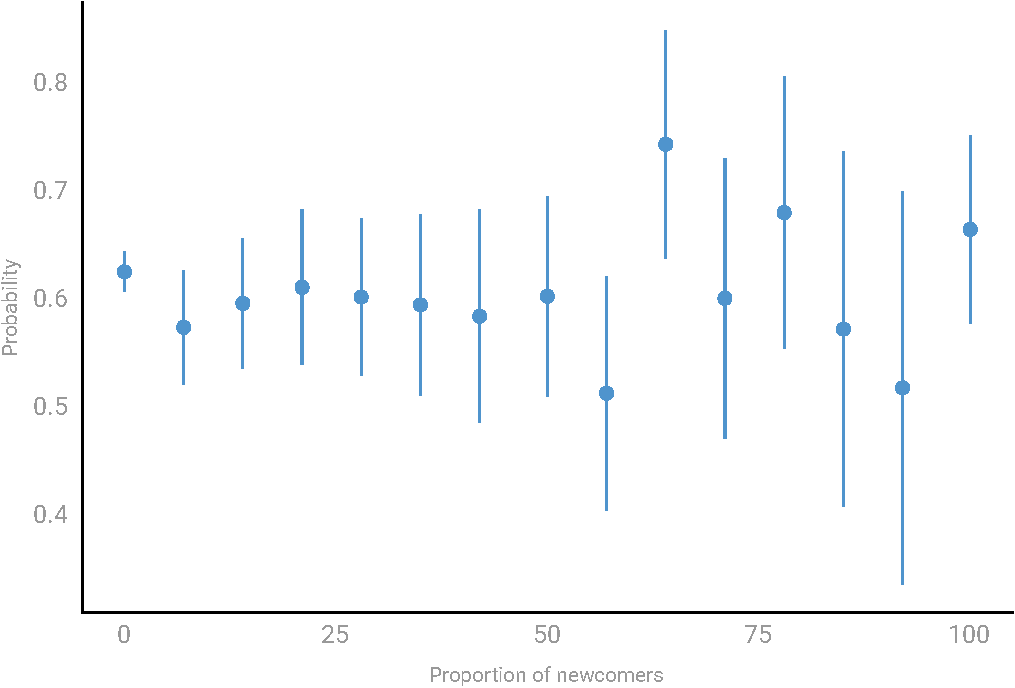
\includegraphics{First_Draft_files/figure-latex/unnamed-chunk-2-1.pdf}

While educational level is not a perfect measure, I argue that it is
reasonable to claim that municipalities staffed by bureaucrats who have
been unable to finish lower school are probably less capable than those
staffed by college-educated bureaucrats. As pointed out by Fukuyama
(2013): ``Beyond taxation, another critical measure of {[}state{]}
capacity is the level of education and professionalization of government
officials.''\footnote{Kohli 2004, Evans 1995.} Other variables could
play a role in the administrative capacity of these municipalities: work
experience, type of contract offered, wages, data which I was able to
gather and process. These will be explored in subsequent research.

A further benefit from measuring educational levels is that it allows
quantifying administrative capacity in an objective manner. It is a
measure that does not rely on expert surveys\footnote{Evans and Rauch
  1999.}, such as the World Governance Indicators constructed by the
World Bank. The study follows a similar research strategy as Bersch et
al. (2015), who analyze different bureaucracies in Brazilian federal
agencies and identify ``islands of excellence'' precisely by measuring
educational levels, types of contracts and partisanship of agency
directors.

\subsection{Motivation:}\label{motivation}

Yet the question remains: why should we look at these municipal
bureaucrats? Indeed, most of the scholarly literature has focused on
national bureaucracies with little discussion of subnational
bureaucracies. This is hardly surprising. From the 1930s to the 1970s,
several Latin American countries had sought to implement
Import-Substitution Industrialization (ISI) as a strategy to develop
economically.\footnote{Love 1994, pp.~402. Hirschmann 1968, pp.~4.} In
doing so, policymakers formulated and implemented economic policy
through a national bureaucracy, usually the Ministry of Finance and a
Central Bank. Centralization of power under military rule further
marginalized municipalities from power.

It was an era characterized by the pursuit of industrialization and the
preeminence of an alliance between technocrats and military
rulers.\footnote{O'Donnell 1979.} Brazil was no exception to these
regional trends.\footnote{O'Donnell 1979.} Within that context, it would
make little sense to analyze municipal bureaucracies, when most (if not
all) of political action took place at the national level.
Decentralization, however, would change that.

Since the enactment of the Constitution of 1988, responsibility for
implementation of different public policies (health provision,
education) has been devolved to Brazilian municipalities.\footnote{Pessoa
  2003, pp.~255.} As a proportion of the national bureaucracy - federal,
state, and municipal - the latter has increased in size and importance
since the 1990s.

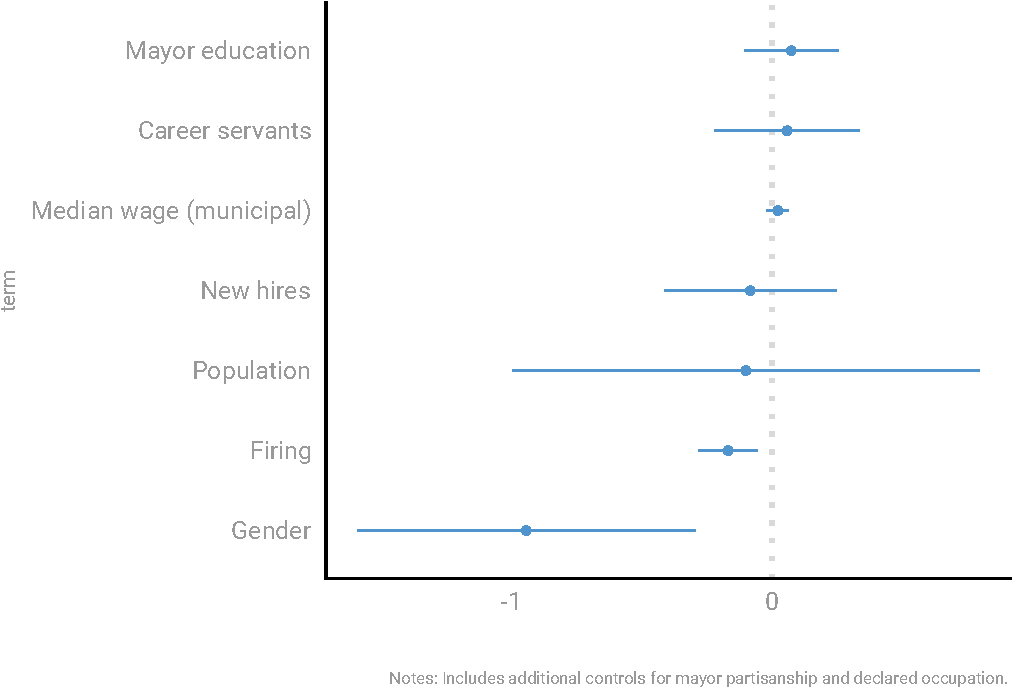
\includegraphics{First_Draft_files/figure-latex/unnamed-chunk-3-1.pdf}

Furthermore, several countries in Latin America are marked by large
within-country heterogeneities. O'Donnell emphasizes that within Latin
American countries, there may be `green areas' with high state capacity
(São Paulo) and large `brown areas' in which it is lower (the Northeast,
Amazon).\footnote{} In countries characterized by large socioeconomic
inequalities, it should not be surprising that there are wide
inequalities in the distribution of
\texttt{state\ capacity".\textbackslash{}footnote\{Hoffman\ and\ Centeno\ 2003\}\ The\ uneven\ spread\ of\ this}capacity"
is a salient feature within these countries, as highlighted by more
recent empirical work.\footnote{Soifer 2015, Bersch et al. 2015}

\end{document}


